\begin{frame}{Computação em nuvem (\textit{Cloud computing})}
	\begin{figure}[htb]
		\centering
		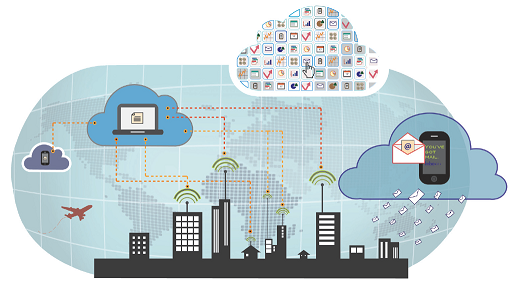
\includegraphics[scale=0.8]{images/cloud-computing-business.png}	
	\end{figure}
\end{frame}

\begin{frame}{Computação em nuvem no cotidiano}
	\begin{figure}[htb]
		\centering
		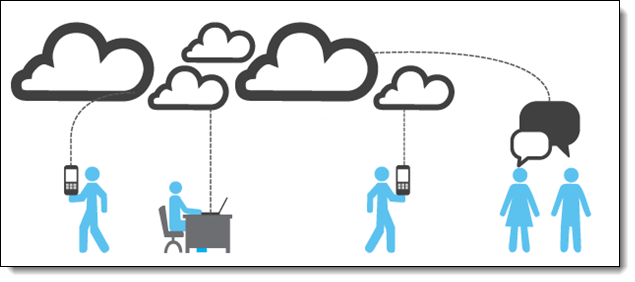
\includegraphics[scale=0.5]{images/cloud-on-life.png}	
	\end{figure}
\end{frame}

\begin{frame}{Uma análise cientométrica de Computação em Nuvem}
	\begin{figure}[htb]
		\centering
		\caption{Percentual de publicação por subárea \cite{Heilig2014}}
		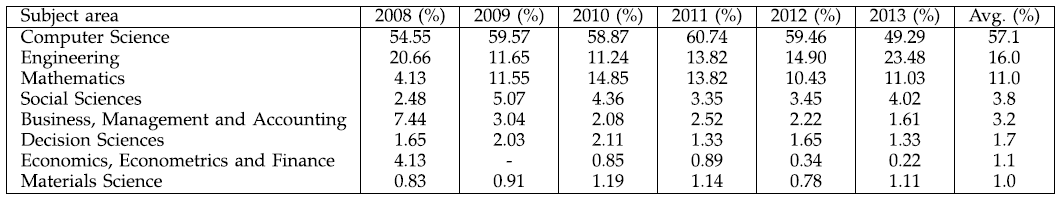
\includegraphics[scale=0.43]{images/sub-area.png}			
	\end{figure}
\end{frame}

\begin{frame}{Uma análise cientométrica de Computação em Nuvem}
	\begin{figure}[htb]
		\centering
		\caption{Palavras chaves (\textit{f} >= 100) \cite{Heilig2014}}
		\includegraphics<1>[scale=0.4]{images/keyword-computing.png}
		\includegraphics<2>[scale=0.4]{images/keyword-computing2.png}
		\includegraphics<3>[scale=0.4]{images/keyword-computing3.png}
	\end{figure}
\end{frame}

\begin{frame}{Contextualização}
	
	\begin{itemize}
		\item Existe uma grande preocupação por parte dos provedores a garantir QoS. Em termos de recursos, significa que os recursos devem ser alocados de forma autônoma sob de manda a responder às influências externas \cite{Padala2007};
		\item Com o crescimento das aplicações intensivas de dados, a dinâmica do sistema passa ser apreciável, tais aplicações tendem a operarem com cargas de trabalho variante no	tempo, causando inúmeras dificuldades \cite{Padala2007}; 		
	\end{itemize}	
	
	\begin{figure}[!htb]
		\centering 
		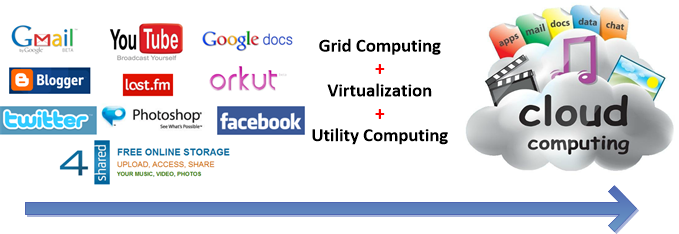
\includegraphics[scale=0.55]{images/cloud-computing.png}
	\end{figure}
	
\end{frame}

\begin{frame}{Contextualização}
	
	\begin{itemize}
		\item A computação em nuvem oferece uma infraestrutura elástica ou escalável que pode ser utilizada para obter recursos; no entanto, um problema em aberto é decidir sobre a correta alocação de recursos ao implantar a nuvem \cite{Cervino2012};		
		\item Este comportamento dinâmico começa a ser apreciado em grande sistemas computacionais, quanto um súbito aumento de requisições para um \textit{website} em que os servidores não conseguem-se ajustar à demanda de modo imediato.
	\end{itemize}	
	
	\begin{figure}[!htb]
		\centering 
		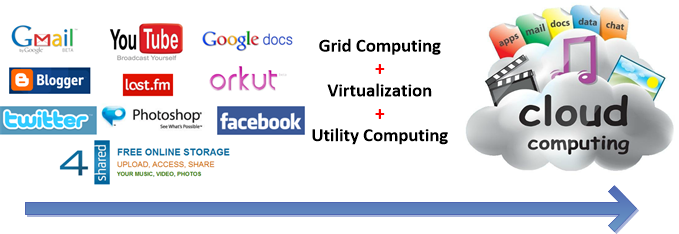
\includegraphics[scale=0.55]{images/cloud-computing.png}
	\end{figure}
	
\end{frame}

\begin{frame}{Dinâmica em um caso real}
	\begin{figure}[htb]
		\centering
		\includegraphics<1>[scale=0.3]{images/grafico-black-friday.jpg}	
		\includegraphics<2>[scale=0.4]{images/grafico-black-friday2.png}	
		\includegraphics<3>[scale=0.4]{images/grafico-black-friday3.png}
		\includegraphics<4>[scale=0.4]{images/grafico-black-friday4.png}
		\caption{Tempo de resposta do \textit{Black Friday} Brasil 2012 \cite{blackfridayNews}}
	\end{figure}
\end{frame}

\begin{frame}{Dinâmica em um caso real}
	\begin{itemize}
		\item  a maioria das aplicações Web são confeccionadas em \textit{mult-tiers} (multi-camadas) devido à flexibilidade de escalabilidade. O planejamento de capacidade para determinar a quantidade de recursos exigido para garantir QoS é uma decisão de longo prazo e quase estático \cite{Dong2014},
		
		\item  a gestão de recursos em tempo real aumenta a sofisticação da arquitetura nos diversos níveis; as dinâmicas emergentes das interligações desses sistemas \textit{mult-tiers} pode produzir efeitos transitórios sobre o desempenho, estes efeitos variáveis no tempo podem potencialmente afetar a capacidade de resposta, eficiência \cite{Lourenco2015}.		
	\end{itemize}
\end{frame}

\begin{frame}{Gerenciamento de recursos}
	GEP PARA MOTIVAÇÂO
\end{frame}	

\begin{frame}{Motivação}

\end{frame}	

\begin{frame}{Objetivo}
	
\end{frame}	